%!TEX program = xelatex
\documentclass[12pt,a4paper]{article}
\usepackage{ctex}
\usepackage{amsmath,amscd,amsbsy,amssymb,latexsym,url,bm,amsthm}
\usepackage{epsfig,graphicx,subfigure}
\usepackage{enumitem,balance,mathtools}
\usepackage{wrapfig}
\usepackage{mathrsfs, euscript}
\usepackage[usenames]{xcolor}
\usepackage{hyperref}
\usepackage{float}
%\usepackage{algorithm}
%\usepackage{algorithmic}
%\usepackage[vlined,ruled,commentsnumbered,linesnumbered]{algorithm2e}
\usepackage[ruled,lined,boxed,linesnumbered]{algorithm2e}

\newtheorem{theorem}{Theorem}[section]
\newtheorem{lemma}[theorem]{Lemma}
\newtheorem{proposition}[theorem]{Proposition}
\newtheorem{corollary}[theorem]{Corollary}
\newtheorem{exercise}{Exercise}[section]
\newtheorem*{solution}{Solution}

\renewcommand{\thefootnote}{\fnsymbol{footnote}}

\newcommand{\postscript}[2]
 {\setlength{\epsfxsize}{#2\hsize}
  \centerline{\epsfbox{#1}}}

\renewcommand{\baselinestretch}{1.0}

\setlength{\oddsidemargin}{-0.365in}
\setlength{\evensidemargin}{-0.365in}
\setlength{\topmargin}{-0.3in}
\setlength{\headheight}{0in}
\setlength{\headsep}{0in}
\setlength{\textheight}{10.1in}
\setlength{\textwidth}{7in}
\makeatletter \renewenvironment{proof}[1][Proof] {\par\pushQED{\qed}\normalfont\topsep6\p@\@plus6\p@\relax\trivlist\item[\hskip\labelsep\bfseries#1\@addpunct{.}]\ignorespaces}{\popQED\endtrivlist\@endpefalse} \makeatother
\makeatletter
\renewenvironment{solution}[1][Solution] {\par\pushQED{\qed}\normalfont\topsep6\p@\@plus6\p@\relax\trivlist\item[\hskip\labelsep\bfseries#1\@addpunct{.}]\ignorespaces}{\popQED\endtrivlist\@endpefalse} \makeatother
\begin{document}
\noindent

%========================================================================
\noindent\framebox[\linewidth]{\shortstack[c]{
\Large{\textbf{CS308 Homework 3}}\vspace{1mm}\\
Exercises for Algorithm Design and Analysis by Li Jiang, 2016 Autumn Semester}}
\begin{center}
\footnotesize{\color{blue} \quad Name:\underline{Gao Chao}  \quad Student ID:\underline {5142029014}\quad Email: \underline {gaoc96@163.com}}
\end{center}

\begin{description}
	\item[Coverage]: Intermediate Code Generation.
\end{description}

\begin{enumerate}
\item (Section 6.1, Exercises 6.1.1) Construct the DAG for the expression

    \begin{center}
    ((x+y)-((x+y)*(x-y)))+((x+y)*(x-y))
    \end{center}


\begin{solution}
\textrm{\\}

construction step
%Your answer should be written here.
\begin{table}[h]
    \centering
    \begin{tabular}{|c|c|}
    \hline
    1) & p1 = Leaf(id, entry-x)\\
    \hline
    2) & p2 = Leaf(id, entry-y)\\
    \hline
    3) & p3 = Node('+', p1, p2)\\
    \hline
    4) & p4 = Leaf(id, entry-x) = p1\\
    \hline
    5) & p5 = Leaf(id, entry-y) = p2\\
    \hline
    6) & p6 = Node('+', p1, p2) = p3\\
    \hline
    7) & p7 = Leaf(id, entry-x) = p1\\
    \hline
    8) & p8 = Leaf(id, entry-y) = p2\\
    \hline
    9) & p9 = Node('-', p1, p2)\\
    \hline
    10) & p10 = Node('*', p3, p9)\\
    \hline
    11) & p11 = Node('-', p3, p10)\\
    \hline
    12) & p12 = Leaf(id, entry-x) = p1\\
    \hline
    13) & p13 = Leaf(id, entry-y) = p2\\
    \hline
    14)& p14 = Node('+', p1, p2) = p3\\
    \hline
    15) & p15 = Leaf(id, entry-x) = p1\\
    \hline
    16) & p16 = Leaf(id, entry-y) = p2\\
    \hline
    17) & p17 = Node('-', p1, p2) = p9\\
    \hline
    18) & p18 = Node('*', p3, p9) = p10\\
    \hline
    19) & p19 = Node('+', p11, p10)\\
    \hline 
    \end{tabular}
    \caption{DAG construction}
    \end{table}
    \textrm{\\}
    DAG
    \begin{figure}[h]
    \center
    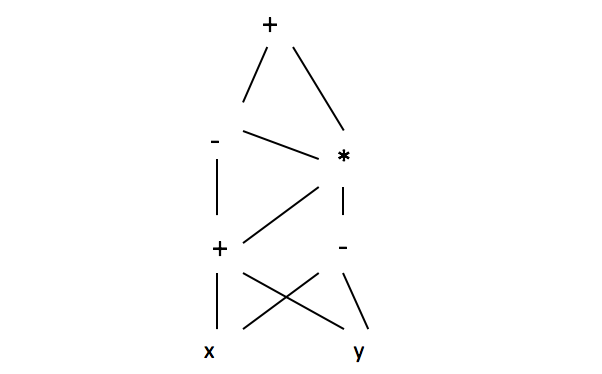
\includegraphics[width=0.8\linewidth]{sol}\vspace{-10pt}
    \caption{DAG} \label{DAG}\vspace{-10pt}
    \end{figure}

\end{solution}

\textrm{\\}
\newpage
\textrm{\\}
\item (Section 6.2, Exercises 6.2.2) Translate the following arithmetic expression into Triples.

    \begin{enumerate}
    \item a = b[i]+c[j]
    \item a[i]=b*c-b*d
    \item x=f(y+1)+2
    \item x=*p+\&y
    \end{enumerate}

\begin{solution}
\textrm{\\}
  \begin{enumerate}
    \item 
    \textrm{\\}
    \begin{table}[h]
    \centering
    \begin{tabular}{|c|c|c|c|}
    \hline
     & op & arg1 & arg2\\
    \hline
    0 & =$[$ $]$ & b & i\\
    \hline
    1 & =$[$ $]$ & c & j\\
    \hline
    2 & + & (0) & (1)\\
    \hline
    3 & = & a & (2)\\
    \hline
    \end{tabular}
    \caption{triple of a = b[i]+c[j]}
    \end{table}
    \newpage
    \item
    \textrm{\\}
    \begin{table}[h]
    \centering
    \begin{tabular}{|c|c|c|c|}
    \hline
     & op & arg1 & arg2\\
    \hline
    0 & * & b & c\\
    \hline
    1 & * & b & d\\
    \hline
    2 & - & (0) & (1)\\
    \hline
    3 & $[$ $]$= & a & i\\
    \hline
    4 & = & (3) & (2)\\
    \hline 
    \end{tabular}
    \caption{triple of a[i]=b*c-b*d}
    \end{table}

    \item 
    \textrm{\\}
    \begin{table}[h]
    \centering
    \begin{tabular}{|c|c|c|c|}
    \hline
     & op & arg1 & arg2\\
    \hline
    0 & + & y & 1\\
    \hline
    1 & param & (0) &  \\
    \hline
    2 & call & f & (1)\\
    \hline
    3 & + & (2) & 2\\
    \hline
    4 & = & x & (3)\\
    \hline 
    \end{tabular}
    \caption{triple of x=f(y+1)+2}
    \end{table}

    \item 
    \textrm{\\}
    \begin{table}[h]
    \centering
    \begin{tabular}{|c|c|c|c|}
    \hline
     & op & arg1 & arg2\\
    \hline
    0 & * & p &  \\
    \hline
    1 & \& & y &  \\
    \hline
    2 & + & (0) & (1)\\
    \hline 
    3 & = & x & (2)\\
    \hline
    \end{tabular}
    \caption{triple of x=*p+\&y}
    \end{table}

  \end{enumerate}

\end{solution}


\end{enumerate}
%========================================================================
\end{document}